\documentclass[compress,xcolor=table]{beamer}
% add handout to optional args for handout version

\usepackage{beamerthemesplit}
\usepackage[utf8]{inputenc}
\usepackage[german]{babel}
\usepackage{german}
\usepackage{graphicx}
\usepackage{subfigure}
\usepackage{epsfig}
\usepackage{tabularx}
\usepackage{latexsym}
\usepackage{url}
\usepackage{tikz}
\usepackage{multimedia}
\usepackage{xcolor}
\usepackage{eso-pic}
\usepackage{color}
\usepackage{type1cm}
\usepackage{listings}
\usepackage{verbatim}
\usepackage{colortbl}
\usepackage{psfrag}
\usepackage{xifthen}
\usepackage[absolute,overlay]{textpos}
\usepackage{palatino}
\usepackage{appendixnumberbeamer}

%% Mulberry Color for highlighting
\definecolor{Mulberry}{cmyk}{0.34,0.90,0,0.02}
\definecolor{Lavender}{cmyk}{0,0.48,0,0}
\definecolor{Melon}{cmyk}{0,0.46,0.50,0}
\definecolor{Peach}{cmyk}{0,0.50,0.70,0}
\definecolor{RedOrange}{cmyk}{0,0.77,0.87,0}
\definecolor{BrickRed}{cmyk}{0,0.89,0.94,0.28}
\definecolor{Mahogany}{cmyk}{0,0.85,0.87,0.35}
\definecolor{BurntOrange}{cmyk}{0,0.51,1,0}
\definecolor{BitterSweet}{cmyk}{0,0.75,1,0.24}
\definecolor{FawkesRed}{rgb}{0.53,0,0}
\definecolor{RosBlue}{rgb}{0.19,0.25,0.38}


\mode<presentation>
{
  \usetheme{FawkesSimple}

  % to hide nav bar uncomment this line
  \setbeamertemplate{navigation symbols}{}

  %\setbeamercovered{transparent}
  \setbeamercovered{%
    again covered={\opaqueness<1->{40}}
  }
}

% Usage notes for handout version:
% Compile the beamer version immediately before you build the handout version,
% otherwise page numbers etc. will be wrong! The .aux files are *not* updated
% in handout mode, see PGF Manual for details why this is necessary.
% Comment out below one of the two pgfuselayout lines for either 2 or 4 slides
% per page. To have a very light grey background uncomment the background canvas
% color line. The logical page options are used to draw borders around each
% slide.
\mode<handout>
{
  \usetheme{Fawkes}

  % to hide nav bar uncomment this line
  \setbeamertemplate{navigation symbols}{}

  %\setbeamercovered{transparent}
  \setbeamercovered{%
    again covered={\opaqueness<1->{40}}
  }

  % Very slight grey background, can be used instead of borders
  %\setbeamercolor{background canvas}{bg=black!5}

  \usepackage{pgfpages}
  \pgfpagesuselayout{4 on 1}[a4paper,border shrink=5mm,landscape]
  %\pgfpagesuselayout{2 on 1}[a4paper,border shrink=5mm]

  \pgfpageslogicalpageoptions{1}{border code=\pgfstroke}
  \pgfpageslogicalpageoptions{2}{border code=\pgfstroke}
  \pgfpageslogicalpageoptions{3}{border code=\pgfstroke}
  \pgfpageslogicalpageoptions{4}{border code=\pgfstroke}
  \nofiles
}


% Declare layers
\pgfdeclarelayer{background}
\pgfsetlayers{background,main} 

% Load PGF libraries
\usetikzlibrary{patterns}
\usetikzlibrary{arrows}
\usetikzlibrary{topaths}
\usetikzlibrary{snakes}
\usetikzlibrary{calc}
\usetikzlibrary{positioning}
\usetikzlibrary{shadows}
\usetikzlibrary{shapes.multipart}


% set lengths for textpos package
\setlength{\TPHorizModule}{10mm}
\setlength{\TPVertModule}{\TPHorizModule}
\textblockorigin{8mm}{16mm} % start everything near the top-left corner
\setbeamercolor{textblock color}{fg=blue!50,bg=white}

\urlstyle{sf}
\urldef{\projecturl}\url{}

%\pgfdeclareimage[width=4cm]{logo-big}{syslife/logo_big}

\institute{%
  %\vspace{1cm}
  \begin{minipage}{\textwidth}\centering
  
\includegraphics[height=0.6cm]{images/rwth-logo}
  \end{minipage}

  \bigskip

  \begin{minipage}{\textwidth}\centering
  \textcolor{FawkesBrown}
  \projecturl
  \end{minipage}
  %\vspace{-1.5cm}
    %  \end{column}
    %\end{columns}
  %\end{minipage}
}


%\titlegraphic{\pgfuseimage{logo-big}}

% \AtBeginPart{\frame{\partpage}}

%numbers=left, numberstyle=\tiny, stepnumber=2, numbersep=5pt
\lstset{language=[GNU]C++,
        basicstyle=\small,
        escapeinside={/*(*/}{/*)*/},
        breaklines=true,
        showstringspaces=false
        }

\lstdefinelanguage{JavaScript}{
  keywords={typeof, new, true, false, catch, function, return, null, catch, switch, var, if, in, while, do, else, case, break},
  keywordstyle=\color{blue}\bfseries,
  ndkeywords={class, export, boolean, throw, implements, import}, %, this
  ndkeywordstyle=\color{darkgray}\bfseries,
  identifierstyle=\color{black},
  sensitive=false,
  comment=[l]{//},
  morecomment=[s]{/*}{*/},
  commentstyle=\color{purple}\ttfamily,
  stringstyle=\color{red}\ttfamily,
  morestring=[b]',
  morestring=[b]"
}

\lstdefinestyle{JSON}
{
  language=JavaScript,
  morekeywords={interface,field,message,comment},
  basicstyle=\footnotesize\ttfamily\vspace{0.2cm},
  breaklines=true,
  showstringspaces=false,
  %keywordstyle=\bfseries,
  keywordstyle=\color{Mulberry},
  frame=lines,
  belowcaptionskip=8pt,
  emphstyle=\itshape,
  numbers=left,
  stepnumber=1,
  backgroundcolor=\color{blue!10},
  rulecolor=\color{blue!50},
  fillcolor=\color{blue!20},
  framexleftmargin=16pt,
  xleftmargin=16pt,
  %stringstyle=\color{BitterSweet},
  stringstyle=\color{BrickRed},
  commentstyle=\color{BrickRed},
  escapechar=\%
  % emph={getup, servo, depends_skills},
  %emphstyle=\underbar,
  %numbers=left,
  %stepnumber=1,
  %%stringstyle=\ttfamily, % typewriter type for strings
}

\lstdefinestyle{SmallJSON}{
  style=JSON,
  basicstyle=\ttfamily\footnotesize,
  numbersep=6pt,
}
\lstdefinestyle{ReallySmallJSON}{
  style=JSON,
  basicstyle=\ttfamily\tiny,
  numbersep=5pt,
}


% Listings stuff
\lstdefinelanguage{Lua}
{
  morekeywords={and,break,do,else,elseif,end,false,for,function,
                if,in,local,nil,not,or,repeat,return,then,true,until,while},
  sensitive=true,
  morecomment=[l]{--},
  morecomment=[s]{--[[}{--]]},
  morestring=[b]{"},
  morestring=[s]{[==[}{]==]},
}

% default style
\lstdefinestyle{Lua}
{
  language=Lua,
  basicstyle=\ttfamily,
  breaklines=true,
  showstringspaces=false,
  %keywordstyle=\bfseries,
  keywordstyle=\color{Mulberry},
  %frame=lines,
  %belowcaptionskip=8pt,
  emphstyle=\itshape,
  %numbers=left,
  stepnumber=1,
  %backgroundcolor=\color{blue!10},
  rulecolor=\color{blue!50},
  fillcolor=\color{blue!20},
  %framexleftmargin=18pt,
  %xleftmargin=18pt,
  stringstyle=\color{BitterSweet},
  %stringstyle=\color{BrickRed},
  commentstyle=\color{BrickRed},
  escapechar=\%
  % emph={getup, servo, depends_skills},
  %emphstyle=\underbar,
  %numbers=left,
  %stepnumber=1,
  %%stringstyle=\ttfamily, % typewriter type for strings
}
\lstdefinestyle{SmallLua}{
  style=Lua,
  basicstyle=\ttfamily\footnotesize,
  numbersep=6pt,
}
\lstdefinestyle{ReallySmallLua}{
  style=Lua,
  basicstyle=\ttfamily\tiny,
  numbersep=5pt,
}

% Default is Lua
\lstset{style=Lua}


% Hyphenation of words with hyphen
\def\hyph{-\penalty0\hskip0pt\relax}


% define an anchor in the frame
\newcommand{\tikzref}[1]{%
  \tikz[remember picture]{%
    \coordinate (#1) at (0,0.5ex);%
  }%
}%


%%% Local Variables: 
%%% mode: latex
%%% TeX-master: "iros2012-robodb"
%%% End: 


\title[Collaborative 3D Model Viewing on the Web]{Collaborative 3D Model Viewing on the Web\\ First Review}
\author[Group 2]{%
  Alexandra Wörner, Dominik Studer, Ali Demiralp\\ Dev Sharma and Frederik Zwilling \\
  \bigskip
  {\scriptsize Group 2}
}

\date[Nov 14th 2014 @ HENM 2014]{Nov 14th 2014 -- First Review HENM}

\begin{document}

\frame[plain]{\titlepage}
\addtocounter{framenumber}{-1}

\begin{frame}
  \frametitle{Overview}
  \tableofcontents[hideallsubsections]
\end{frame}
%\addtocounter{framenumber}{-1}

\section{Project Description}

\begin{frame}
  \frametitle{At a Glance}
  \begin{columns}
    \begin{column}{0.8\textwidth}
      \begin{description}[]
        \item[Why Collaborative 3D Model Viewing?] \hfill \\
        \begin{itemize}
          \item Teaching and learning from 3D models more comprehensive than from 2D drawing
          \item Access to real objects costly or limited
          \item Collaborative viewing allows new, interactive learning methods
        \end{itemize}

        \bigskip
        \item[Our Approach] \hfill \\
          \begin{itemize}
            \item Upload models (especially from 3D scanning) into a database
            \item View models in a browser on different devices
            \item Manipulate view on all devices at the same time
        \end{itemize}
      \end{description}
    \end{column}

    \begin{column}{0.2\textwidth}
      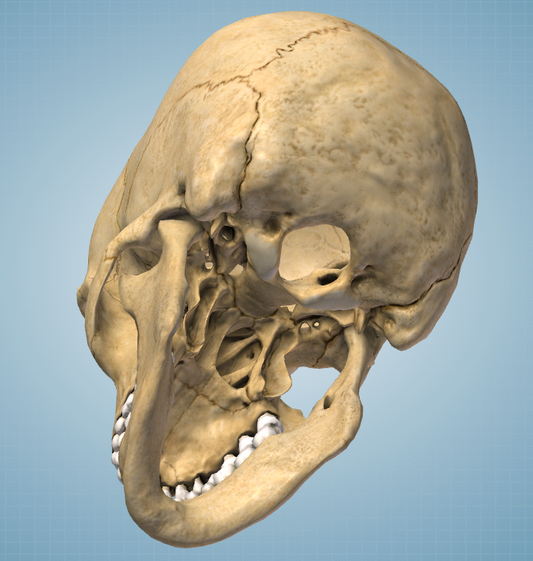
\includegraphics[width=.9\textwidth]{images/skull}\\
      \bigskip
      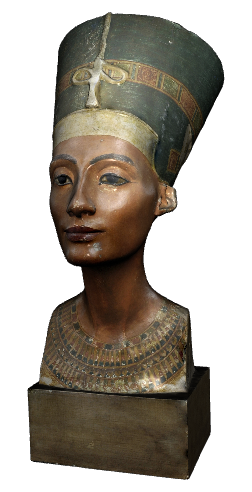
\includegraphics[width=.9\textwidth]{images/nefertiti}
    \end{column}
  \end{columns}
\end{frame}

\section{Technology survey}

\begin{frame}
  \frametitle{Technology Survey - Digitization of Physical Objects}
  \begin{columns}
    \begin{column}{0.7\textwidth}
      \begin{description}[]
        \item[White Light Scanner] \hfill \\
        \begin{itemize}
          \item Allows digitization of small objects
          \item Scanning process requires user interaction
          \item As accurate as a laser scanner
        \end{itemize}
       	\item[Structure From Motion] \hfill \\
       	\begin{itemize}
       	  \item Creates 3-D models from videos!
       	  \item Utilizes modern computer vision techniques
       	  \item No user interaction necessary
       	  \item Output is not nearly accurate as WLS
       	\end{itemize}
      \end{description}
   	\end{column} 	
   	\begin{column}{0.3\textwidth}
   	  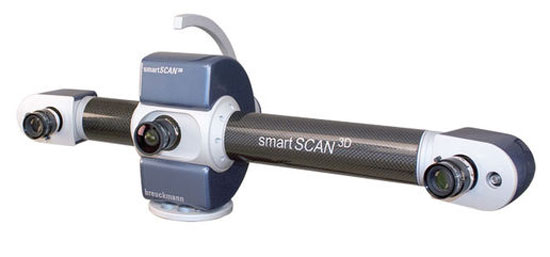
\includegraphics[width=1\textwidth]{images/scanner}\\
   	  \bigskip
   	  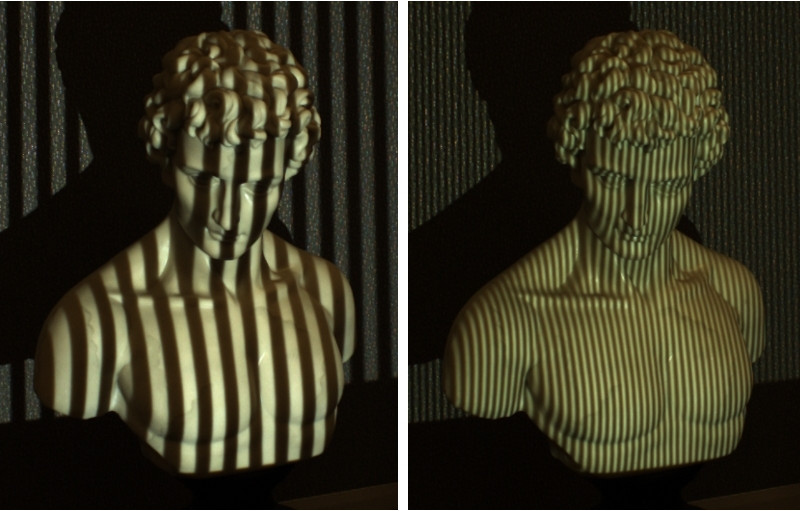
\includegraphics[width=1\textwidth]{images/light_scan}\\
   	  \bigskip
   	  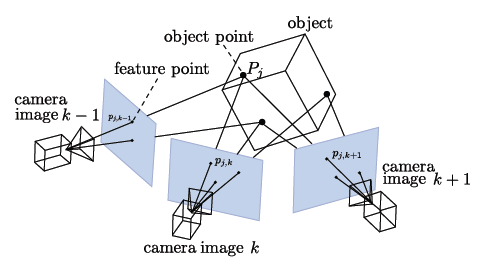
\includegraphics[width=1\textwidth]{images/sfm}\\
   	\end{column}
  \end{columns}	
\end{frame}

\begin{frame}
  \frametitle{Technology Survey - Image and Model Data Storage}
  \begin{columns}
    \begin{column}{0.8\textwidth}
      \begin{description}[]
        \item[Database - To Embrace or Avoid?] \hfill \\
        \begin{itemize}
          \item Model files are generally massive
          \item Indexing them is not trivial
          \item ACID (Atomicity, Consistency, Isolation, Durability)
          \item Authorization
        \end{itemize}
        \item[Candidates] \hfill \\
        \begin{itemize}
          \item MongoDB
          \item PostgreSQL
          \item MySQL
        \end{itemize}
      \end{description}  
    \end{column} 	
    \begin{column}{0.2\textwidth}
      
\includegraphics[width=.9\textwidth]{images/mongo}\\
      \bigskip
      
\includegraphics[width=.9\textwidth]{images/postgresql}\\
      \bigskip
      
\includegraphics[width=.9\textwidth]{images/mysql}\\
    \end{column}
  \end{columns}	
\end{frame}

\begin{frame}
  \frametitle{Technology Survey - 3D Data Presentation}
  \begin{columns}
    \begin{column}{0.7\textwidth}
      \begin{description}[]
        \item[Criteria] \hfill \\
        \begin{itemize}
          \item Supports common 3-D data formats
          \item Allows user to apply affine transformations
          \item Exposes internal state to the browser
          \item Final product is not dependent on an add-on.
        \end{itemize}
        \item[Candidates] \hfill \\
        \begin{itemize}
          \item Three.js
          \item O3D
          \item X3Dom
        \end{itemize}
      \end{description}  
    \end{column} 	
    \begin{column}{0.3\textwidth}
      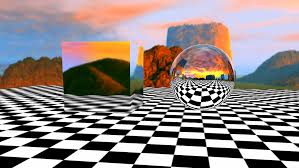
\includegraphics[width=1\textwidth]{images/scene}\\
      \bigskip
      \bigskip
      \bigskip
      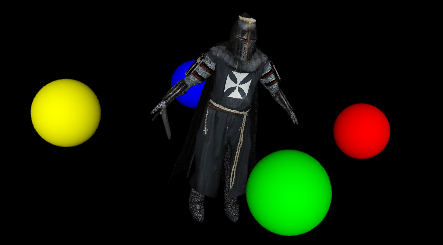
\includegraphics[width=1\textwidth]{images/model}\\
    \end{column}
  \end{columns}	
\end{frame}

\begin{frame}
  \frametitle{Technology Survey - Cross-Browser Communication}
  \begin{columns}
    \begin{column}{0.7\textwidth}
      \begin{description}[]
        \item[Role SDK] \hfill \\
        \begin{itemize}
          \item Open source e-learning environment 
          \item Personalized with widgets
          \item Any web-application is convertible to a widget with some preamble
          \item Provides multi-user interaction
        \end{itemize}
        \item[Inter-Widget Communication System] \hfill \\
        \begin{itemize}
          \item Defined as part of the preamble
          \item Communicates with other add-ons in the same space
          \item Publishes events to all active users in the same learning space
        \end{itemize}
      \end{description}  
    \end{column} 	
    \begin{column}{0.3\textwidth}
      
\includegraphics[width=1\textwidth]{images/role}\\
      \bigskip
      \bigskip
      \bigskip
      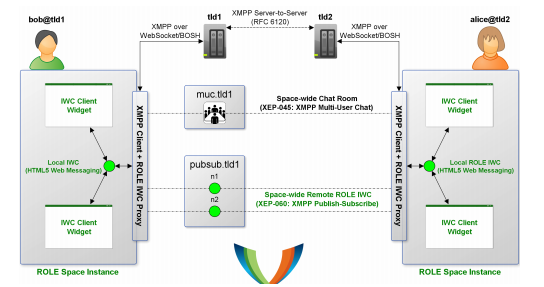
\includegraphics[width=1\textwidth]{images/iwc}\\
    \end{column}
  \end{columns}	
\end{frame}

\section{Market analysis}

\begin{frame}
  \frametitle{Market analysis}
 \begin{columns}
    \begin{column}{0.6\textwidth}
      \begin{description}[]
        \item[Industrial Diversity] \hfill \\
        \begin{itemize}
          \item Medical industry, Architecture, Computer Graphics, TV, movies, video games.
          \item Educational sector.
        \end{itemize}

        \item[Wide User base] \hfill \\
          \begin{itemize}
            \item Everyone with a mobile device or desktop computer that supports the used technology.
            \item 75\% of desktop computers and 50\% of mobile devices are equipped with WebGL-enabled browsers.
        \end{itemize}
      \end{description}
    \end{column}

    \begin{column}{0.5\textwidth}
      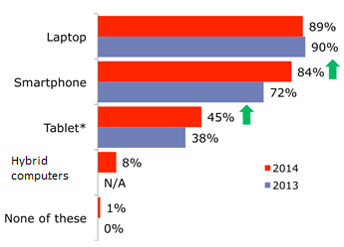
\includegraphics[width=.9\textwidth]{images/devices.png}\\
    \end{column}
  \end{columns}
\end{frame}

\begin{frame}
  \frametitle{Market analysis}
      \begin{description}[]
        \item[Industry cost structure] \hfill \\
        \begin{itemize}
          \item Scanning equipment is expensive, but will become more affordable.
          \item Standardized web technologies and SDKs.
        \end{itemize}

        \item[Distribution Channels] \hfill \\
          \begin{itemize}
            \item Medical Faculty at RWTH Aachen.
            \item Expand to more medical faculties in Germany and  broaden the scope of application.
        \end{itemize}

\item[Key Success Factors] \hfill \\
          \begin{itemize}
            \item Adjust to new technology/developments.
           \item Abilities in programming.
	\item Building reputation.
\end{itemize}
\end{description}
\end{frame}

\section{Gantt Chart}

\begin{frame}
  \frametitle{Gantt Chart}
A Gantt chart is a bar chart that shows the tasks of a project, when each task must take place and how long each will take.  
  \begin{description}[]
	\item[Conventions] \hfill \\
	\begin{itemize}
	\item Try to keep it simple.
          \item Highlight milestones/reviews.
        \item Assign different colours to team members .
        \item Indicate the (temporal) dependency of one task from another with arrows.
      \end{itemize}
 \end{description}
\end{frame}


\begin{frame}
  \frametitle{Gantt Chart}
  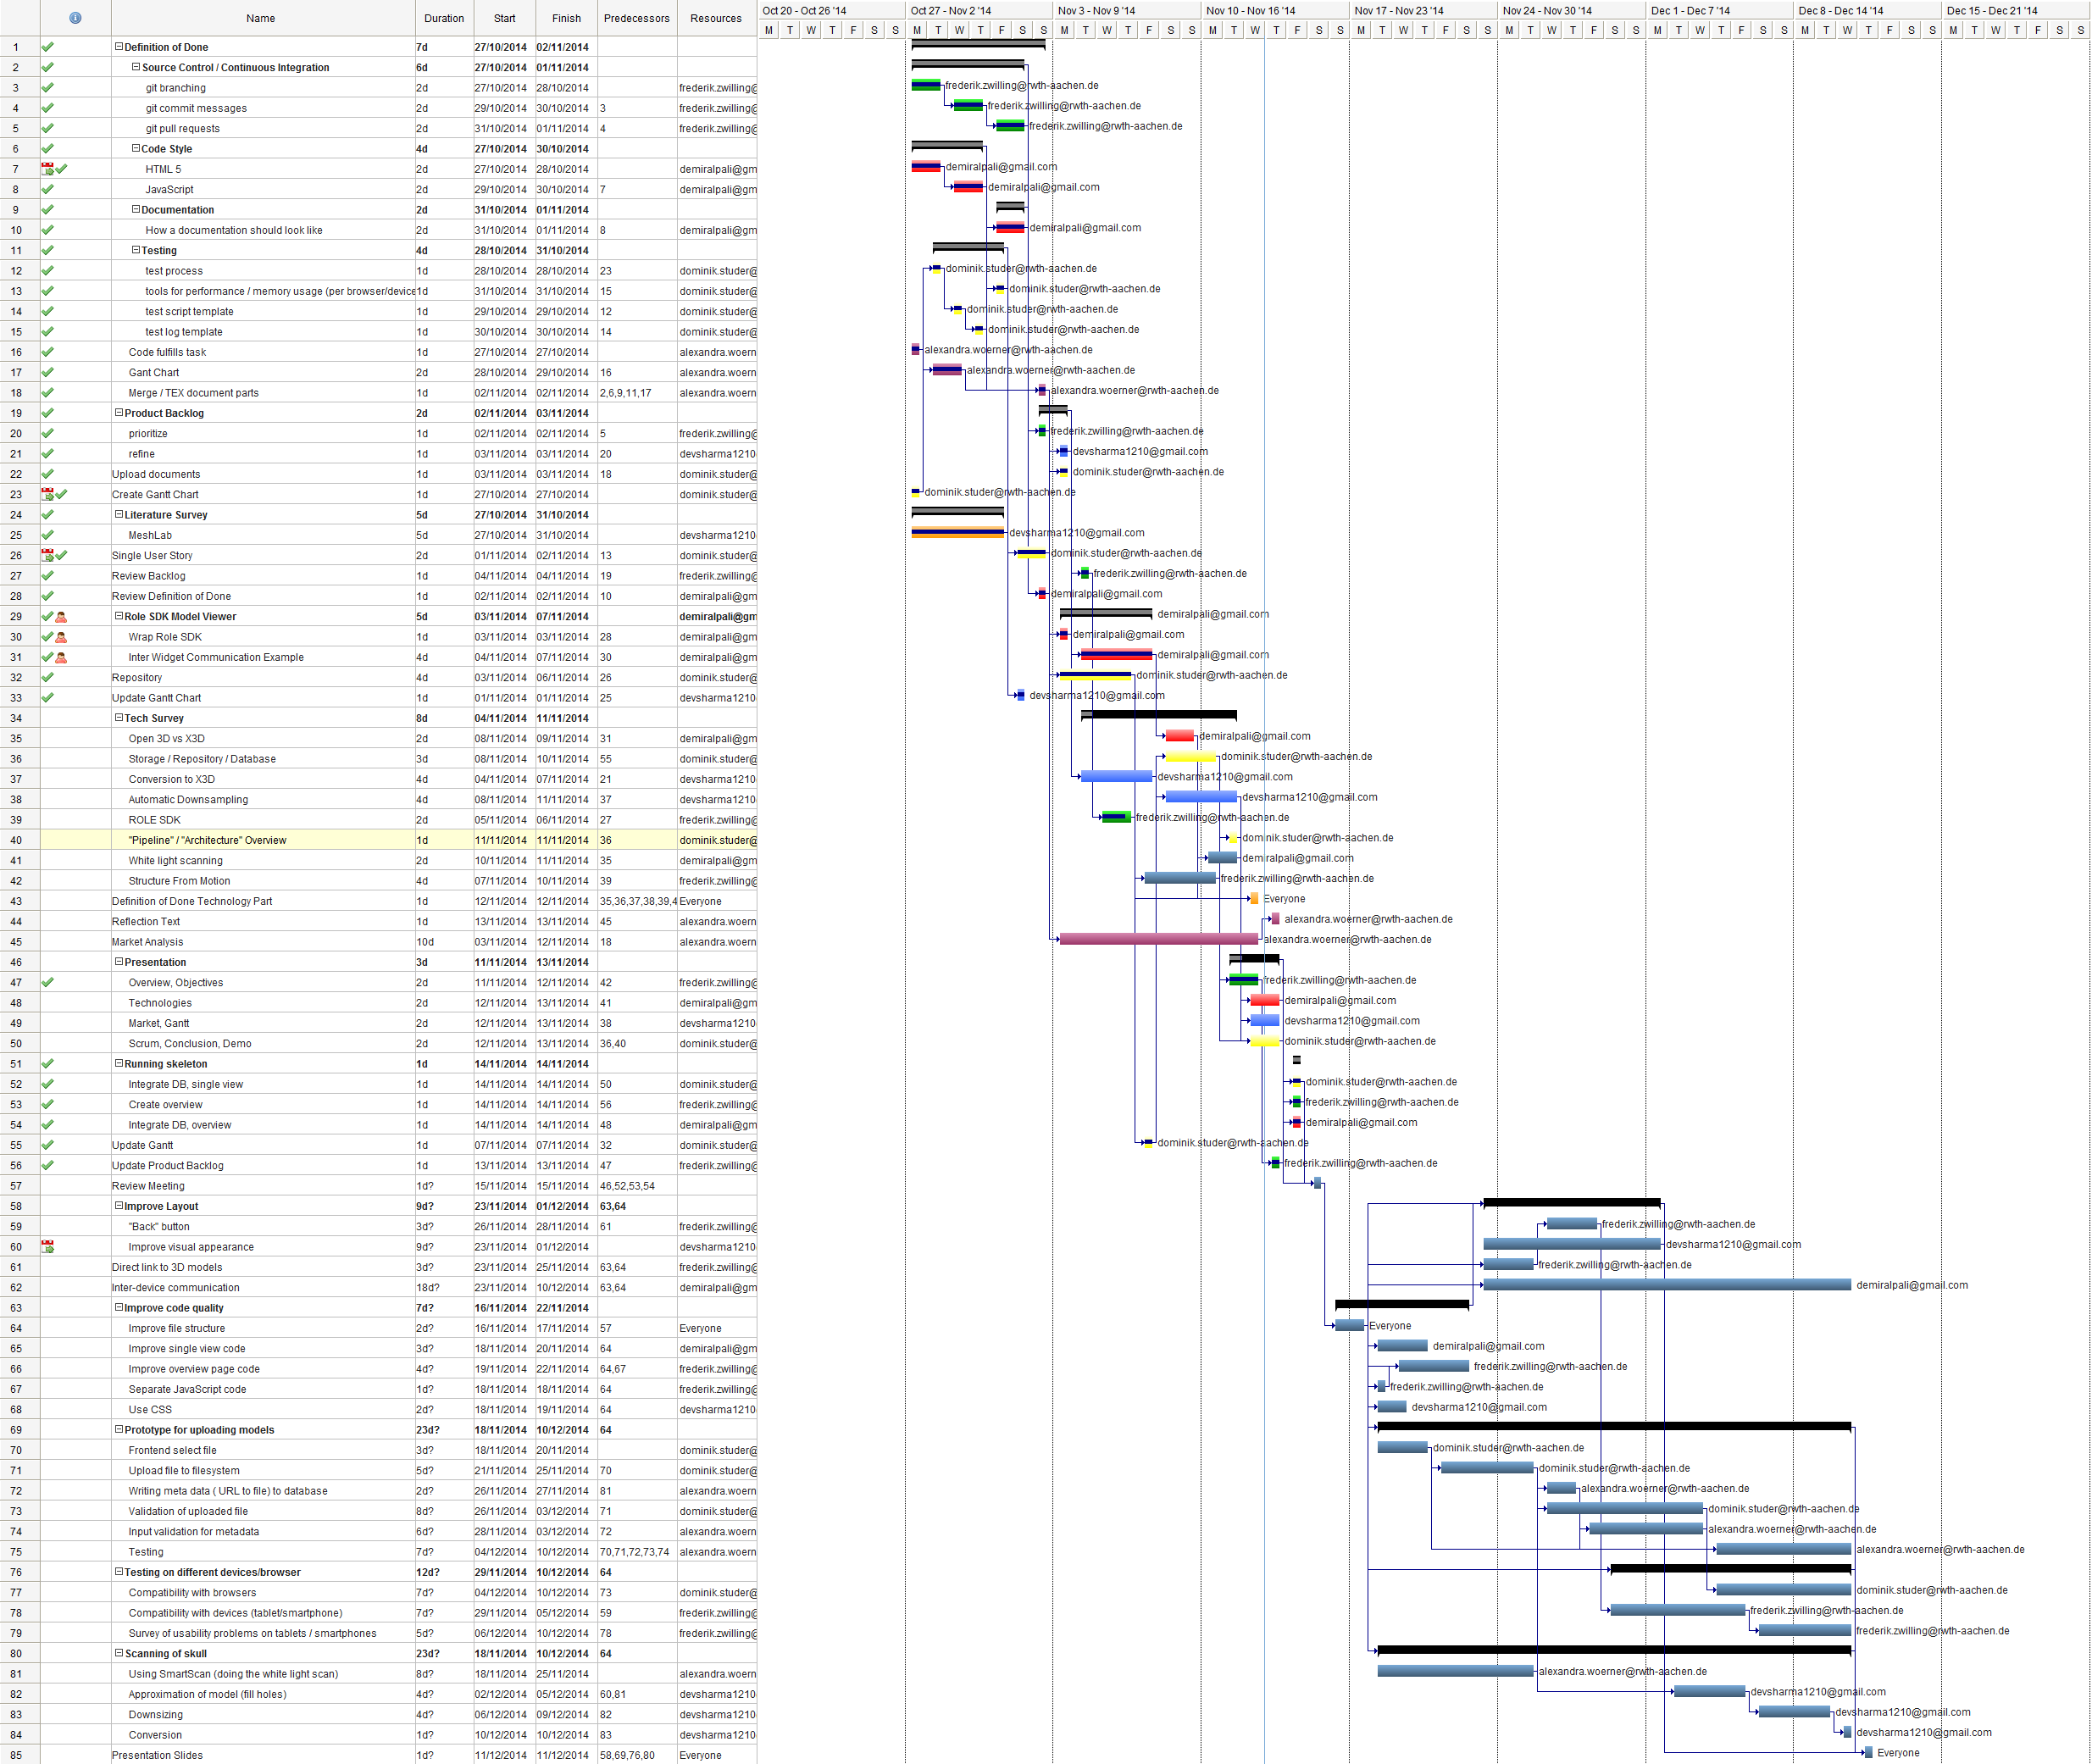
\includegraphics[width=1.2\textwidth, height=0.7\textwidth]{images/gantt_chart.png}\\
\end{frame}

\section{Scrum, Team process}

\begin{frame}
  \frametitle{Scrum}
  \begin{description}[]
    \item[Customer contact] \hfill \\
    \begin{itemize}
      \item 3 Customer meetings in first 2 weeks
      \item Mail
    \end{itemize}
  \end{description}
  \begin{description}[]
    \item[Collaborative working] \hfill \\
    \begin{itemize}
      \item Sprint Planning
      \item Daily Scrum: 1x each week
      \item Sprint Review: Customer currently not available
	   \item Sprint Retrospective: To be introduced
    \end{itemize}
  \end{description}
\end{frame}

\begin{frame}
  \frametitle{Reflection on team process}
  \begin{description}[]
    \item[Team member] \hfill \\
    \begin{itemize}
      \item Evaluation of skills and preferences
      \item Distribution of roles
    \end{itemize}
  \end{description}
  \begin{description}[]
    \item[Communication] \hfill \\
    \begin{itemize}
      \item Meetings, Facebook
      \item Sharing results of technology survey: mailing list
    \end{itemize}
  \end{description}
  \begin{description}[]
    \item[Collaborative working] \hfill \\
    \begin{itemize}
      \item Product Backlog, DoD, Market Analysis, ..: Google Drive
      \item Protocols of customer meetings
    \end{itemize}
  \end{description}
\end{frame}

\section{Demo}

\begin{frame}
  \frametitle{Demo of current prototype}
%  \begin{description}[]
%    \item[{\fontsize{50}{48} \selectfont Demo}] \hfill \\
%  \end{description}
  
\includegraphics[width=\textwidth]{images/demo}
\end{frame}

\section{Conclusion}

\begin{frame}
  \frametitle{Conclusion and next steps}
  \begin{description}[]
    \item[Conclusion] \hfill \\
    \begin{block}{}
      \centering\textbf{
        \begin{itemize}
          \item Collaborative viewing of 3D models
          \item Access to limited objects, new learning methods
          \item The educational sector and many industries offer great potential and profitability for usage of 3D models.
        \end{itemize}
      }
    \end{block}
    \item[Next Steps] \hfill \\
      \begin{itemize}
        \item Talking with the customer
        \item Interface for uploading models
        \item Inter-device-communication
        \item Layout prototype
      \end{itemize}
  \end{description}  
\end{frame}

\end{document}
